\section{Introduction}

In the realm of 3D computer graphics, the objective is to portray a three-dimensional environment on a flat screen, which inherently possesses only two dimensions. 
Even in the realm of stereoscopic imagery, the illusion of depth arises from the brain's processing of distinct 2D images presented to each eye. 
Utilizing geometrical primitives, 3D computer graphics encapsulates objects within a three-dimensional realm, subsequently rendering a 2D depiction of this space for display on the screen.

The process of generating a 2D image from a 3D scene is known as projection. 
This technique defines the 2D depiction of a 3D object by the intersection of a set of projection rays with a surface.

Typically, this surface is a plane known as the projection plane. On this plane, a rectangular area corresponds to the screen.
An essential characteristic of planar projections is that linear segments in the 3D scene maintain their straightness when projected onto the screen.
It's important to note that this characteristic no longer holds true when projections are made onto surfaces other than a plane.

Because the projected segments link the projections of their endpoints, it's enough to project the vertices and connect them to reconstruct a 2D representation of the corresponding 3D objects.

We will consider two types of planar projections:
\begin{itemize}
    \item \textit{Parallel projection}: all rays are parallel to the same direction.
    \item \textit{Perspective projection}: all the rays pass through a point, called the center of projection.
\end{itemize}
\begin{figure}[H]
    \centering
    \begin{subfigure}{0.49\textwidth}
        \centering
        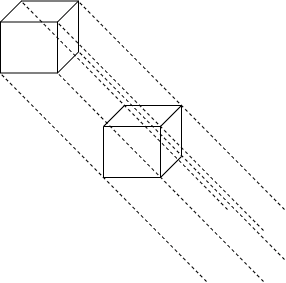
\includegraphics[width=0.4\linewidth]{images/parallel.png} 
        \caption{Parallel}
    \end{subfigure}
    \begin{subfigure}{0.49\textwidth}
        \centering
        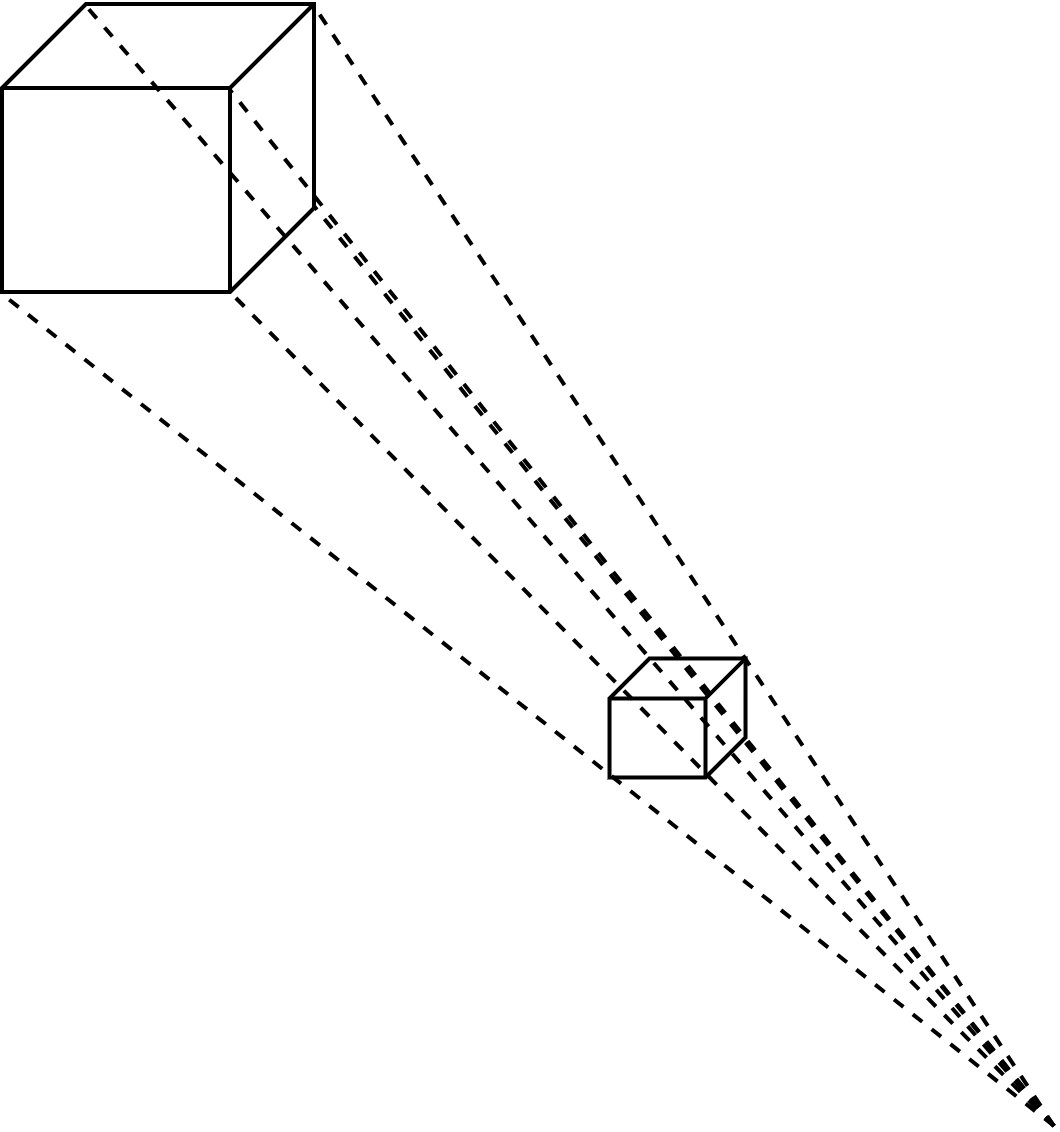
\includegraphics[width=0.4\linewidth]{images/perspective.png}
        \caption{Perspective}
    \end{subfigure}
    \caption{Types of projections}
\end{figure}
In both parallel and perspective projections, a point on the screen corresponds to an infinite number of coordinates in space. 
This results directly from losing a component when transitioning from a 3D spatial system to a 2D screen system.

\paragraph*{Properties}
In parallel projections, all points that lie along a line parallel to the projection ray are projected onto the same pixel.
In perspective projection, all points that align with both the projected pixel and the center of projection are mapped to the same location.

\paragraph*{From the world to the screen}
In 3D computer applications, projections are realized by converting 3D coordinates between two reference systems. Specifically, projections transform world coordinates into 3D normalized screen coordinates.

The coordinate system that describes objects in 3D space is known as World Coordinates (or global coordinates).

World Coordinates represent a right-handed Cartesian coordinate system, where the origin is mapped to the center of the screen. 
In the $y$-up version considered in this course, the $x$ and $y$-axes align with the horizontal and vertical edges of the screen, respectively. 
The $z$-axis extends out of the screen, toward the viewer.

It's worth noting that certain applications, such as Blender, employ a different convention for World Coordinates known as $z$-up. 
In this case, the z-axis aligns with the vertical screen direction, and the y-axis points inside the screen.
Some applications may even use a left-handed system, where the y-axis extends toward the viewer.
\begin{figure}[H]
    \centering
    \begin{subfigure}{0.49\textwidth}
        \centering
        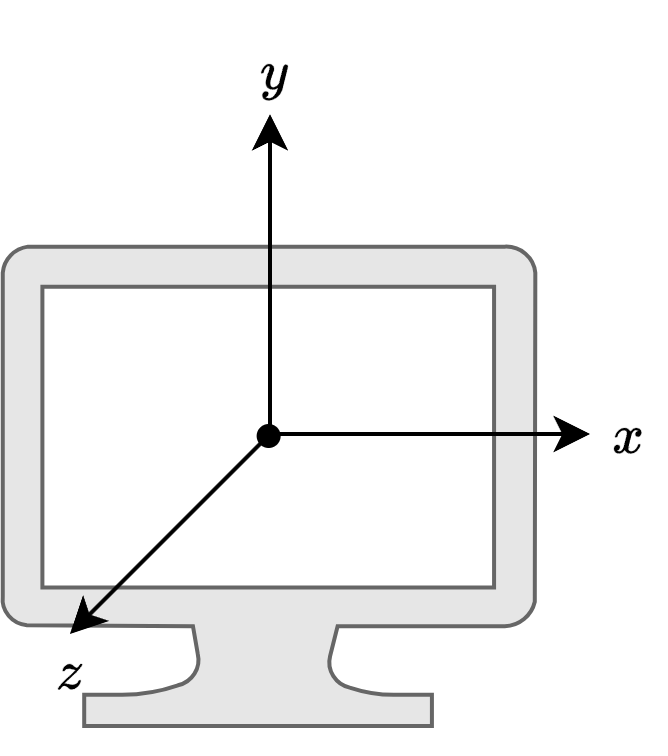
\includegraphics[width=0.4\linewidth]{images/yup.png} 
        \caption{$y$-up}
    \end{subfigure}
    \begin{subfigure}{0.49\textwidth}
        \centering
        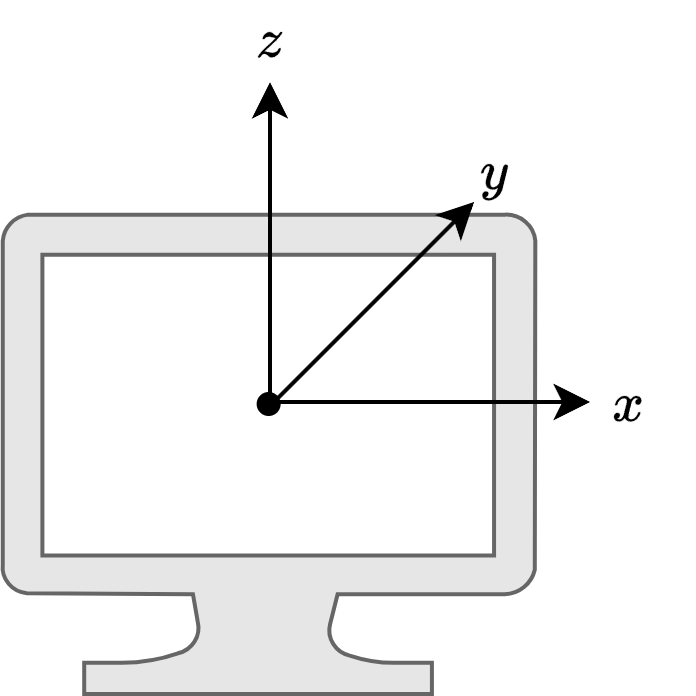
\includegraphics[width=0.4\linewidth]{images/zup.png}
        \caption{$z$-up}
    \end{subfigure}
    \caption{World coordinates}
\end{figure}
As previously discussed, Normalized Screen Coordinates provide a means to specify point positions on a screen or window in a device-independent manner.

Despite the screen being a 2D surface, pixels originating from 3D images require a distance from the viewer to correctly sort surfaces and avoid generating unrealistic images.

In 3D Normalized Screen Coordinates, a third component is introduced, which, in the context of Vulkan, falls within the $[0,1]$ range. 
Points with smaller z-values are considered closer to the viewer. 
It's important to note that in this context, all normalized screen coordinates are considered to be 3D.

It's worth mentioning that other low-level graphics engines, such as OpenGL, employ completely different systems for normalized screen coordinates.